\documentclass[a4paper,10pt]{article}
\usepackage{fontspec}
\setmainfont{Times New Roman}
\usepackage[left=1.2cm, right=1.2cm, top=1.5cm, bottom=1.5cm]{geometry}
\usepackage{enumitem}
\usepackage{titlesec}
\usepackage{xcolor}
\usepackage{hyperref}
\usepackage{graphicx}
\usepackage{tabularx}
\usepackage{ulem}
\usepackage{booktabs}
\usepackage{fontawesome5}
\usepackage{marvosym}
\usepackage{parskip}

\hypersetup{
    colorlinks=true,
    linkcolor=black,
    filecolor=black,
    urlcolor=blue,
}

\titleformat{\section}{\Large\bfseries\color{black}}{}{0em}{}
\titleformat{\subsection}{\bfseries}{}{0em}{}
\setlist[itemize]{leftmargin=*, noitemsep, topsep=1pt, parsep=0pt}
\renewcommand{\arraystretch}{1.2}

\begin{document}
\raggedbottom
\titlespacing{\section}{0pt}{6pt}{3pt}
\titlespacing{\subsection}{0pt}{4pt}{2pt}
\linespread{1.1}

\noindent
\begin{tabular}{m{3cm} l}
    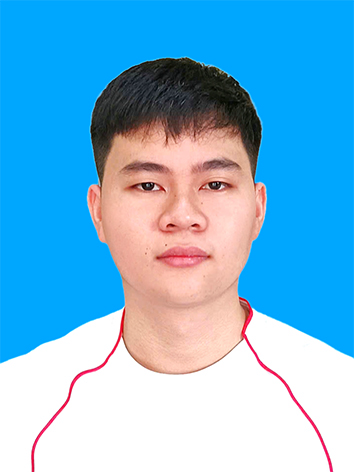
\includegraphics[width=3cm, height=3.5cm]{image.png} &
    \begin{tabular}{@{}l}
        \multicolumn{1}{c}{\textbf{\LARGE Nguyễn Hữu Lộc} \quad \textbf{\large Fresher Backend Developer}} \\[10pt]
        \begin{tabular}{@{}ll@{}}
            \faEnvelope & \href{mailto:lockbkbang@gmail.com}{\uline{lockbkbang@gmail.com}} \\
            \faPhone & 0397845443 \\
            \faBirthdayCake & 23/09/2004 \\
        \end{tabular}
        \hspace{20pt}
        \begin{tabular}{@{}ll@{}}
            \faMapMarker & Hoc Mon, TP HCM \\
            \faGithub & \href{https://github.com/LocNguyenSGU}{\uline{https://github.com/LocNguyenSGU}} \\
            \faGlobe & \href{https://locnguyensgu.github.io/nguyenhuuloc2k4/}{\uline{https://locnguyensgu.github.io/nguyenhuuloc2k4/}} \\
        \end{tabular}
    \end{tabular}
\end{tabular}

\section{Mục tiêu nghề nghiệp}
\vspace{-10pt}
\noindent\rule{\linewidth}{0.5pt}
Sinh viên năm cuối ngành Công nghệ Thông tin, định hướng phát triển ở mảng backend. Mong muốn tìm kiếm vị trí \textbf{Fresher Backend Developer} để vận dụng kiến thức đã học vào các dự án thực tế, tiếp tục rèn luyện tư duy xây dựng hệ thống và đóng góp hiệu quả cho đội ngũ phát triển sản phẩm.

\section{Học vấn}
\vspace{-10pt}
\noindent\rule{\linewidth}{0.5pt}
\begin{tabularx}{\linewidth}{l X}
    \textbf{09/2022 - 02/2026} & \textbf{Đại học Sài Gòn} \\
    & Cử nhân Công nghệ Thông tin \\
    & GPA: 3.38/4.0 (8.26/10) \\
    & Học bổng khuyến khích học tập: 5 lần
\end{tabularx}

\section{Thành tích}
\vspace{-8pt}
\noindent\rule{\linewidth}{0.5pt}
\begin{itemize}
    \item \textbf{Top 2 Hackathon 02/2025 (Đại học Sài Gòn)}: Phát triển trợ lý học tập ứng dụng \textbf{OpenAI API}; phụ trách phần backend và hoàn thiện bản demo hoạt động trong 24 giờ.
    \item \textbf{Bài báo nghiên cứu}: \textit{Adaptive Learning Optimization for Reinforcement Learning}, công bố và trình bày trực tiếp tại \textbf{FJCAI 2026} (Hội thảo về Trí tuệ Nhân tạo Quốc tế 2026).
    \item \textbf{Khóa luận tốt nghiệp}: Xây dựng hệ thống AI tích hợp Moodle, đạt điểm \textbf{10/10}.
\end{itemize}

\section{Kỹ năng}
\vspace{-10pt}
\noindent\rule{\linewidth}{0.5pt}
\renewcommand{\arraystretch}{1.1}
\begin{tabularx}{\linewidth}{l X}
    \textbf{Ngôn ngữ:} & Java, Ruby \\
    \textbf{Frameworks:} & Spring Boot, Ruby on Rails, ReactJS \\
    \textbf{Cơ sở dữ liệu:} & MySQL, Redis, MongoDB, PostgreSQL \\
    \textbf{Kiến trúc:} & Microservices, MVC \\
    \textbf{Giao tiếp thời gian thực:} & WebSocket \\
    \textbf{Công cụ / DevOps:} & Git/GitHub, Docker, AWS Cloud, n8n
\end{tabularx}

\section{Dự án}
\vspace{-10pt}
\noindent\rule{\linewidth}{0.5pt}

\subsection*{1. Internal System \hfill \small (Dự án nhóm - 5 thành viên)}
\begin{itemize}
    \item \textbf{Thời gian:} 09/2025 - 09/2026
    \item \textbf{Mô tả:} Hệ thống quản lý đơn hàng, nhân viên, khách hàng và sản phẩm cho doanh nghiệp thương mại điện tử, được xây dựng theo kiến trúc \textbf{MVC} và sử dụng \textbf{PostgreSQL}.
    \item \textbf{Vai trò chính:}
    \begin{itemize}
        \item Phát triển các chức năng backend cho phân hệ đơn hàng, phục vụ khối lượng hơn \textbf{5.000+ đơn/ngày}.
        \item Xây dựng tính năng thu thập và xử lý dữ liệu giá sản phẩm từ các sàn thương mại điện tử với tệp CSV lớn \textbf{100.000+ dòng}, sử dụng \textbf{Sidekiq} để xử lý bất đồng bộ và lưu trữ vào \textbf{PostgreSQL}.
        \item Thực hiện migration dữ liệu từ hai cơ sở dữ liệu riêng biệt về một hệ thống lưu trữ thống nhất, xử lý tập dữ liệu phức tạp với quy mô \textbf{500.000+ dòng}.
        \item Phát triển công cụ trích xuất thông tin từ hóa đơn có cấu trúc phức tạp, đạt độ chính xác \textbf{97\%} khi tích hợp API của \textbf{Gemini AI}.
        \item Xây dựng luồng tự động qua \textbf{MCP} và bot đăng sản phẩm, hỗ trợ đăng \textbf{1.000 sản phẩm/ngày}, áp dụng cơ chế giới hạn theo từng sản phẩm cùng các thao tác \textbf{create, retrieve, update} để tăng hiệu quả vận hành.
    \end{itemize}
    \item \textbf{Công nghệ:} Ruby, MVC, PostgreSQL, Redis, Docker, AWS EC2, Sidekiq
\end{itemize}

\subsection*{2. Hệ thống tạo nội dung SEO \hfill \small (Dự án nhóm - 3 thành viên)}
\begin{itemize}
    \item \textbf{Thời gian:} 12/2024 - 06/2025
    \item \textbf{Mô tả:} Hệ thống hỗ trợ tạo nội dung SEO tự động, phân tích xu hướng và xuất bản bài viết lên website.
    \item \textbf{Vai trò chính:}
    \begin{itemize}
        \item Thiết kế kiến trúc hệ thống và cơ sở dữ liệu phục vụ quy trình tạo nội dung.
        \item Xây dựng luồng xử lý xu hướng và sinh bài viết tự động bằng \textbf{OpenAI API} và \textbf{DeepSeek}, sau đó đăng bài lên website thông qua \textbf{Shopify GraphQL}.
        \item Thiết lập workflow với \textbf{n8n} và cơ chế cập nhật thời gian thực bằng \textbf{WebSocket}.
        \item Tối ưu quy trình sản xuất nội dung hằng ngày với tỷ lệ người dùng chấp nhận bài viết khoảng \textbf{80\%}, đồng thời hỗ trợ tăng khoảng \textbf{20\%} lượng truy cập SEO cho website.
    \end{itemize}
    \item \textbf{Công nghệ:} Ruby, OpenAI API, DeepSeek, Shopify GraphQL, n8n, WebSocket
\end{itemize}

\end{document}
